% Copyright 2026 Sreeram Anil
% SPDX-License-Identifier: CC-BY-4.0
% =============================================================================
%  Interacting multiple model estimator
% =============================================================================
\chapter{Interacting multiple model estimator (IMM)}
\label{ch:imm}

\section*{At a glance}
\begin{tabular}{@{}l>{\raggedright\arraybackslash}p{0.76\textwidth}@{}}
Family & Adaptive Kalman \\
Header & \texttt{include/estkit/filters/imm.hpp} \\
Registered name & \texttt{IMM} \\
State dimension & $n_x = 4$ (cell model), $r = 3$ modes --- generic in $n_x,n_u,n_y$ and in $r$ (template \texttt{int NM}) \\
Cost per step & $r\times$ EKF $+\ \mathcal{O}(r^2 n_x^2)$ mixing; $\approx 2080$\,ns/step, $r(n_x+n_x^2)$ extra reals, no heap \\
Primary references & \cite{blom1988imm,barshalom2001,lijilkov2005mm,magill1965mmae,jazwinski1970} \\
\end{tabular}

\section{Motivation and aerospace/BMS relevance}
Every filter in this chapter so far infers a \emph{scalar} summary of what is wrong --- a noise
variance, a covariance inflation --- from a single innovation sequence.  The recurring failure is
that the sequence does not contain enough information to say \emph{what} changed: a noisier sensor
and a wrong model both inflate the innovations, and the adaptive filters of
\cref{ch:sagehusaakf}, \cref{ch:iaeakf} and \cref{ch:vbakf} always blame the sensor while the strong tracking filter of
\cref{ch:stf} always blames the model.  On the \texttt{noise\_step} scenario the STF is $20\times$
worse than the EKF precisely because it makes the wrong attribution.

The interacting multiple model estimator resolves the ambiguity by carrying the competing
hypotheses explicitly.  A bank of $r$ filters runs in parallel, each with a different assumed
operating regime, and the data decide --- through the likelihood of each filter's innovation --- how
much each hypothesis is worth.  Blom and Bar-Shalom \cite{blom1988imm} added the ingredient that
makes it practical: the modes are allowed to \emph{switch} according to a Markov chain, and the
filters are re-initialised at every step from a mixture of all of them.  The result is an estimator
that costs $r$ filters but behaves like a bank of $r^k$ hypothesis-history filters; it is the
standard tool in manoeuvring-target tracking \cite[Sec.~11.6]{barshalom2001}\cite{lijilkov2005mm}
and in aerospace fault detection.

For a battery pack the natural modes are operating regimes rather than manoeuvres: (i) nominal,
(ii) the voltage sense channel has become noisy (inverter switching, a marginal connector, an
intermittent multiplexer), (iii) the cell no longer matches its stored model (ageing, temperature
excursion, a different cell chemistry after a module swap).  The IMM produces, as a by-product, the
posterior probability of each regime --- a directly usable health signal that none of the single
filters can provide.

\section{Problem statement and assumptions}
The plant is \eqref{eq:sh:proc}--\eqref{eq:sh:meas} with a mode variable
$m_k\in\{1,\dots,r\}$ that selects the noise statistics:
\begin{equation}
\mQ^{(j)}(\vx,\vu) = q_j\,\mQ(\vx,\vu),\qquad
\mR^{(j)}(\vx,\vu) = \varrho_j\,\mR(\vx,\vu),\qquad j = 1,\dots,r,
\label{eq:imm:modes}
\end{equation}
with design constants $q_j,\varrho_j>0$.  The dynamics $f$ and the output map $h$ are the same in
every mode.
\begin{assumption}\label{as:imm:markov}
$\{m_k\}$ is a first-order Markov chain with known, time-invariant transition probabilities
$\pi_{ij} = \mathrm{Pr}\{m_k=j\mid m_{k-1}=i\}$, $\sum_j\pi_{ij}=1$, independent of the state.
\end{assumption}
\begin{assumption}\label{as:imm:gauss}
Conditioned on a mode \emph{history}, the state posterior is Gaussian; the IMM approximates the
mixture over histories by a single Gaussian per mode (the "merging" approximation of
\cite{blom1988imm}).
\end{assumption}

\section{Derivation}
The exact Bayesian filter for a Markov-switching system requires one Gaussian per mode
\emph{sequence}, hence $r^k$ of them at time $k$.  The IMM keeps $r$ of them and re-merges once per
cycle.  Write $\mu_{k}^{(j)} = \mathrm{Pr}\{m_k=j\mid\vy_{1:k}\}$ for the mode probabilities and
$\big(\xhat^{(j)}_{k},\mP^{(j)}_{k}\big)$ for the mode-conditioned moments.

\subsection{Step 1 --- mixing probabilities}
By the total probability theorem and \cref{as:imm:markov}, the predicted mode probability is
\begin{equation}
\bar c_j = \mathrm{Pr}\{m_k=j\mid\vy_{1:k-1}\} = \sum_{i=1}^{r}\pi_{ij}\,\mu^{(i)}_{k-1},
\label{eq:imm:cbar}
\end{equation}
and the probability that the system was in mode $i$ at $k-1$ \emph{given} that it is in mode $j$ at
$k$ is, by Bayes' rule,
\begin{equation}
\mu^{(i|j)}_{k-1} = \mathrm{Pr}\{m_{k-1}=i\mid m_k=j,\ \vy_{1:k-1}\} = \frac{\pi_{ij}\,\mu^{(i)}_{k-1}}{\bar c_j}.
\label{eq:imm:mix}
\end{equation}

\subsection{Step 2 --- mixed initial conditions}
The prior for filter $j$ at time $k-1$ is the mixture
$\sum_i \mu^{(i|j)}_{k-1}\,\N{\xhat^{(i)}_{k-1}}{\mP^{(i)}_{k-1}}$.  Matching its first two moments
(this is \cref{as:imm:gauss}) gives
\begin{align}
\xhat^{0(j)}_{k-1} &= \sum_{i=1}^{r}\mu^{(i|j)}_{k-1}\,\xhat^{(i)}_{k-1}, \label{eq:imm:x0}\\
\mP^{0(j)}_{k-1} &= \sum_{i=1}^{r}\mu^{(i|j)}_{k-1}\Big[\mP^{(i)}_{k-1}
   + \big(\xhat^{(i)}_{k-1}-\xhat^{0(j)}_{k-1}\big)\big(\xhat^{(i)}_{k-1}-\xhat^{0(j)}_{k-1}\big)^\T\Big].
\label{eq:imm:P0}
\end{align}
The rank-one spread terms in \eqref{eq:imm:P0} are what makes the IMM more than a bank of
independent filters: a mode whose estimate disagrees with the others receives an inflated
covariance and therefore a larger gain, so it can catch up.  This is also the reason the IMM
improves the \emph{nominal} mode's behaviour even when that mode carries almost all the
probability --- see the benchmark discussion.

\subsection{Step 3 --- mode-matched filtering}
Each filter runs a complete EKF cycle from $\big(\xhat^{0(j)}_{k-1},\mP^{0(j)}_{k-1}\big)$ with its
own noise scalings:
\begin{align}
\xhat^{-(j)}_k &= f(\xhat^{0(j)}_{k-1},\vu_{k-1}), &
\mP^{-(j)}_k &= \mF\mP^{0(j)}_{k-1}\mF^\T + q_j\mQ, \label{eq:imm:pred}\\
\bm{e}^{(j)}_k &= \vy_k - h(\xhat^{-(j)}_k,\vu_k), &
\mS^{(j)}_k &= \mH\mP^{-(j)}_k\mH^\T + \varrho_j\mR, \label{eq:imm:innov}\\
\mK^{(j)}_k &= \mP^{-(j)}_k\mH^\T\big(\mS^{(j)}_k\big)\inv, &
\xhat^{(j)}_k &= \xhat^{-(j)}_k + \mK^{(j)}_k\bm{e}^{(j)}_k, \label{eq:imm:upd}
\end{align}
with a Joseph-form covariance update.  The Jacobians $\mF,\mH$ are evaluated at the respective
mode's own linearisation point.

\subsection{Step 4 --- mode likelihoods}
Under \cref{as:imm:gauss} the innovation of filter $j$ is Gaussian with covariance $\mS^{(j)}_k$, so
the likelihood of mode $j$ given the new measurement is
\begin{equation}
\Lambda^{(j)}_k = p\big(\vy_k\mid m_k=j,\ \vy_{1:k-1}\big)
= \big|2\pi\mS^{(j)}_k\big|^{-1/2}\exp\!\Big(\!-\tfrac12\,\bm{e}^{(j)\T}_k\big(\mS^{(j)}_k\big)\inv\bm{e}^{(j)}_k\Big).
\label{eq:imm:lik}
\end{equation}

\subsection{Step 5 --- mode probability update}
Bayes' rule with the predicted probabilities \eqref{eq:imm:cbar} as prior:
\begin{equation}
\mu^{(j)}_k = \frac{\Lambda^{(j)}_k\,\bar c_j}{\sum_{l=1}^{r}\Lambda^{(l)}_k\,\bar c_l}.
\label{eq:imm:mu}
\end{equation}
Note that no weight can vanish permanently: even if $\mu^{(j)}_{k-1}=0$, \eqref{eq:imm:cbar} gives
$\bar c_j\ge \pi_{ij}\mu^{(i)}_{k-1}>0$.  The Markov chain is the IMM's built-in protection against
the hypothesis lock-out that afflicts the static bank of \cref{ch:mmae}.

\subsection{Step 6 --- combination}
The output is the moment-matched mixture
\begin{align}
\xhat_k &= \sum_{j=1}^{r}\mu^{(j)}_k\,\xhat^{(j)}_k, \label{eq:imm:xout}\\
\mP_k &= \sum_{j=1}^{r}\mu^{(j)}_k\Big[\mP^{(j)}_k + \big(\xhat^{(j)}_k-\xhat_k\big)\big(\xhat^{(j)}_k-\xhat_k\big)^\T\Big].
\label{eq:imm:Pout}
\end{align}
\eqref{eq:imm:xout}--\eqref{eq:imm:Pout} are used for output only; the mode-conditioned moments are
what is carried forward.

\section{Algorithm}
\begin{algorithm}[H]
\caption{IMM --- one sampling period}
\begin{algorithmic}[1]
\Require $\{\xhat^{(j)}_{k-1},\mP^{(j)}_{k-1},\mu^{(j)}_{k-1}\}_{j=1}^{r}$, $\bm\Pi$, $\vu_{k-1},\vy_k,\vu_k$
\State \textbf{Mixing:} $\bar c_j\gets\sum_i\pi_{ij}\mu^{(i)}_{k-1}$;\quad $\mu^{(i|j)}\gets\pi_{ij}\mu^{(i)}_{k-1}/\bar c_j$
\State \textbf{Mixed ICs:} $\xhat^{0(j)}\gets\sum_i\mu^{(i|j)}\xhat^{(i)}_{k-1}$;\quad
       $\mP^{0(j)}\gets\sum_i\mu^{(i|j)}[\mP^{(i)}_{k-1}+\bm\delta^{(i,j)}\bm\delta^{(i,j)\T}]$,\ $\bm\delta^{(i,j)}=\xhat^{(i)}_{k-1}-\xhat^{0(j)}$
\State \textbf{Time update} of every mode: \eqref{eq:imm:pred}
\State \textbf{(predicted measurement for the host: } $\yhat_k=\sum_j\bar c_j\,h(\xhat^{-(j)}_k,\vu_k)$\textbf{)}
\State \textbf{Measurement update} of every mode: \eqref{eq:imm:innov}--\eqref{eq:imm:upd}, Joseph form, constrain
\State \textbf{Log-likelihoods:} $\ell_j\gets-\tfrac12\big[\bm{e}^{(j)\T}\mS^{(j)-1}\bm{e}^{(j)}+\ln\det\mS^{(j)}+n_y\ln2\pi\big]$ via the Cholesky factor of $\mS^{(j)}$
\State \textbf{Mode update:} $\mu^{(j)}\gets\bar c_j\exp(\ell_j-\max_l\ell_l)$, normalise, floor at $\mu_{\min}$, renormalise
\State \textbf{Combination:} \eqref{eq:imm:xout}--\eqref{eq:imm:Pout}
\Ensure $\xhat_k,\mP_k,\{\mu^{(j)}_k\}$
\end{algorithmic}
\end{algorithm}

\paragraph{Numerical form of the likelihood.}  \eqref{eq:imm:lik} is never evaluated directly.  For
the cell model $\det\mS\approx4\times10^{-6}$ and the exponent can reach $-10^3$, which underflows
in single precision.  The implementation computes $\ell_j$ from the Cholesky factor
$\mL\mL^\T=\mS^{(j)}$ ($\ln\det\mS = 2\sum_i\ln L_{ii}$, quadratic form by forward substitution) and
subtracts $\max_l\ell_l$ before exponentiating, so the mode update is exact up to round-off in both
the double and the float32 build.

\paragraph{Timing convention.}  The benchmark adapter calls \texttt{predict($\vu_{k-1}$)},
\texttt{predict\_measurement($\vu_k$)}, \texttt{update($\vy_k,\vu_k$)}.  Mixing (steps 1--2) is done
at the start of \texttt{predict()}, so it happens exactly once per cycle; the predicted measurement
is the mixture over modes weighted by the \emph{predicted} probabilities $\bar c_j$, which is the
correct one-step-ahead predictive mean under \cref{as:imm:gauss}.

\section{Application to the battery model}
\label{sec:imm:bank}
$r=3$ modes over the same \texttt{EcmModel}:
\begin{center}
\begin{tabular}{@{}lll>{\raggedright\arraybackslash}p{0.6\textwidth}@{}}
\toprule
mode & $q_j$ & $\varrho_j$ & interpretation \\
\midrule
1 & $1$   & $1$   & nominal: the identified model and the datasheet sensor noise are right \\
2 & $1$   & $100$ & degraded voltage channel: $\sigma_v$ ten times nominal \\
3 & $100$ & $100$ & gross model mismatch: neither the transition nor the output model is trustworthy \\
\bottomrule
\end{tabular}
\end{center}
with $\pi_{ii}=1-(r-1)p$, $\pi_{ij}=p$ and $p=10^{-4}$, i.e.\ an expected mode dwell time of
$1/(2p)=5000$ samples $=\SI{500}{\second}$ --- one to two flight phases, which is the right order for
a fault that persists rather than flickers.  $\varrho_2=100$ is chosen to bracket the
\texttt{noise\_step} fault ($\SI{2}{\milli\volt}\to\SI{20}{\milli\volt}$ is a factor $92$ in
variance once the current-sensor feed-through is included) and, more generally, to represent "the
voltage channel is an order of magnitude worse than specified".  $q_3=100$ represents "the cell has
drifted from its model", and it is deliberately paired with $\varrho_3=100$ rather than with
$\varrho_3=1$.

That pairing is a deviation from the naive "high $\mQ$ only" third hypothesis and it is worth
justifying, because the benchmark makes the case sharply.  A pure high-$\mQ$ mode responds to model
error by trusting the \emph{voltage} more.  On this cell that is the wrong response whenever the
mismatch is itself a voltage error --- which it usually is, because ageing raises $R_0$ and the ECM's
dominant unmodelled term at any appreciable current is $\Delta R_0\,i$.  Measured on
\texttt{aged\_cell}, the bank $\{(1,1),(1,100),(100,1)\}$ gave $\mathrm{rmse}=3.75\,\%$ and
$\mathrm{rmse}_{ss}=3.71\,\%$ in the single-seed development sweep, worse than the plain EKF;
replacing mode 3 by $(100,100)$ gave $0.51\,\%$ / $0.58\,\%$, and the final three-seed run confirms
the choice at $0.66\,\%$ / $0.83\,\%$ against the EKF's $1.18\,\%$ / $1.52\,\%$.  Intermediate pairings
$(100,\varrho_3)$ with $\varrho_3\in\{3,10,30\}$ interpolate monotonically between the two.  The
$(100,100)$ hypothesis is therefore the honest one for this plant: "when the model is wrong, so is
the output equation".  An $r=4$ bank containing both was also tried and is worse on
\texttt{aged\_cell} ($3.18\,\%$ / $3.22\,\%$) because the extra hypothesis draws probability away from
the useful one.

\section{Implementation notes}
\begin{itemize}[leftmargin=1.4em]
\item \textbf{One model instance.}  The modes differ only in the scalars $q_j,\varrho_j$, so the bank
      shares a single \texttt{Model} object.  The memory overhead over a single EKF is
      $r(n_x+n_x^2)+r^2+3r$ reals $=0.6$\,kB for the cell model, instead of the
      $\approx 12$\,kB that $r$ full filter objects (each holding a copy of the
      241-point OCV table) would cost.
\item \textbf{Stack.}  The mixing step needs $r$ temporary states and $r$ temporary covariances;
      these are plain arrays in the stack frame of \texttt{predict()} ($480$\,bytes for
      $r=3$, $n_x=4$), so there is still no heap allocation anywhere.
\item \textbf{Mode-probability floor.}  $\mu_{\min}=10^{-6}$ is applied after normalisation purely as
      a numerical guard; the Markov mixing already prevents lock-out, as noted after
      \eqref{eq:imm:mu}.
\item \textbf{Cost.}  Measured \SI{2076}{\nano\second}/step against \SI{478}{\nano\second}/step for
      the EKF --- $4.3\times$, i.e.\ $r$ filters plus about $45\,\%$ for mixing and combination.  On a
      \SI{400}{\mega\hertz} Cortex-M7 this is roughly \SI{27}{\micro\second}/step; at \SI{10}{\hertz}
      and one filter per cell, a 96-cell pack would need about \SI{2.6}{\milli\second} per sample, a
      $3\,\%$ duty cycle --- feasible, but four times a plain EKF, which is a reason to run the IMM
      only on the weakest cells of a pack.
\item \textbf{float32.}  The log-domain mode update makes the filter insensitive to precision; the
      single-precision build reproduces the double-precision metrics to three digits and diverges on
      no scenario.
\item \textbf{Limitations.}  The transition matrix is a design parameter that the data do not
      identify; $p$ trades reaction speed against mode chattering.  The bank can only represent
      hypotheses that were put into it, and the merging approximation \eqref{eq:imm:P0} is exact only
      when the mode-conditioned posteriors are genuinely Gaussian.
\end{itemize}

\section{Benchmark results}
% Copyright 2026 Sreeram Anil
% SPDX-License-Identifier: CC-BY-4.0
\begin{table}[H]\centering\footnotesize\setlength{\tabcolsep}{4pt}
\caption{IMM: cell-level benchmark on the eVTOL mission (mean over seeds; RMSE and max error in \% SOC; $t_\mathrm{conv}$: first time the error stays below 2\,\% for 60\,s, -- = never; EKF reference: steady-state RMSE of the plain EKF on the same data).}\label{tab:cell_IMM}
\begin{tabular}{llrrrrrcrr}\toprule
plant & scenario & RMSE & RMSE$_\mathrm{ss}$ & max & $t_\mathrm{conv}$ [s] & RMSE$_v$ [mV] & div. & EKF ref. & ns/step \\ \midrule
ECM & nominal & 0.18 & 0.04 & 1.03 & 0 & 0.79 & no & 0.05 & 2076 \\
ECM & init\_error & 0.16 & 0.04 & 1.69 & 0 & 2.13 & no & 0.05 & 2077 \\
ECM & current\_bias & 0.55 & 0.62 & 1.35 & 0 & 0.86 & no & 0.61 & 2058 \\
ECM & noise\_step & 0.18 & 0.05 & 1.03 & 0 & 1.05 & no & 0.12 & 2082 \\
ECM & outliers & 0.18 & 0.08 & 1.94 & 0 & 0.93 & no & 0.21 & 2075 \\
ECM & cold & 0.24 & 0.18 & 1.09 & 0 & 1.90 & no & 0.16 & 2064 \\
ECM & hot & 0.19 & 0.03 & 0.98 & 0 & 0.54 & no & 0.03 & 2063 \\
ECM & aged\_cell & 0.66 & 0.83 & 1.96 & 0 & 4.48 & no & 1.52 & 2058 \\
ECM & param\_mismatch & 0.88 & 0.96 & 1.24 & 0 & 3.32 & no & 1.36 & 2065 \\
ECM & sensor\_dropout & 0.18 & 0.05 & 1.03 & 0 & 1.68 & no & 0.46 & 2058 \\
ECM & preisach & 0.70 & 0.20 & 2.08 & 73 & 0.82 & no & 0.20 & 2060 \\
ECM & combined & 2.20 & 1.02 & 8.01 & 833 & 5.45 & no & 12.44 & 2080 \\
\midrule
SPM & nominal & 2.77 & 2.81 & 3.47 & 0 & 1.10 & no & 3.73 & 1965 \\
SPM & init\_error & 3.04 & 3.03 & 3.85 & 29 & 2.21 & no & 3.81 & 1963 \\
SPM & current\_bias & 3.69 & 4.35 & 4.89 & 0 & 1.23 & no & 5.69 & 1959 \\
SPM & noise\_step & 2.79 & 2.85 & 3.47 & 0 & 1.94 & no & 3.30 & 2003 \\
SPM & outliers & 2.12 & 2.25 & 2.38 & 0 & 1.19 & no & 1.99 & 1962 \\
SPM & cold & 2.41 & 2.22 & 3.19 & 20 & 5.29 & no & 7.35 & 1941 \\
SPM & hot & 2.10 & 2.17 & 2.48 & 0 & 0.70 & no & 2.16 & 1921 \\
SPM & param\_mismatch & 2.25 & 2.41 & 2.55 & 0 & 2.31 & no & 3.13 & 1958 \\
SPM & sensor\_dropout & 1.62 & 1.60 & 2.31 & 0 & 1.99 & no & 5.31 & 1965 \\
\bottomrule\end{tabular}\end{table}

\begin{figure}[H]\centering
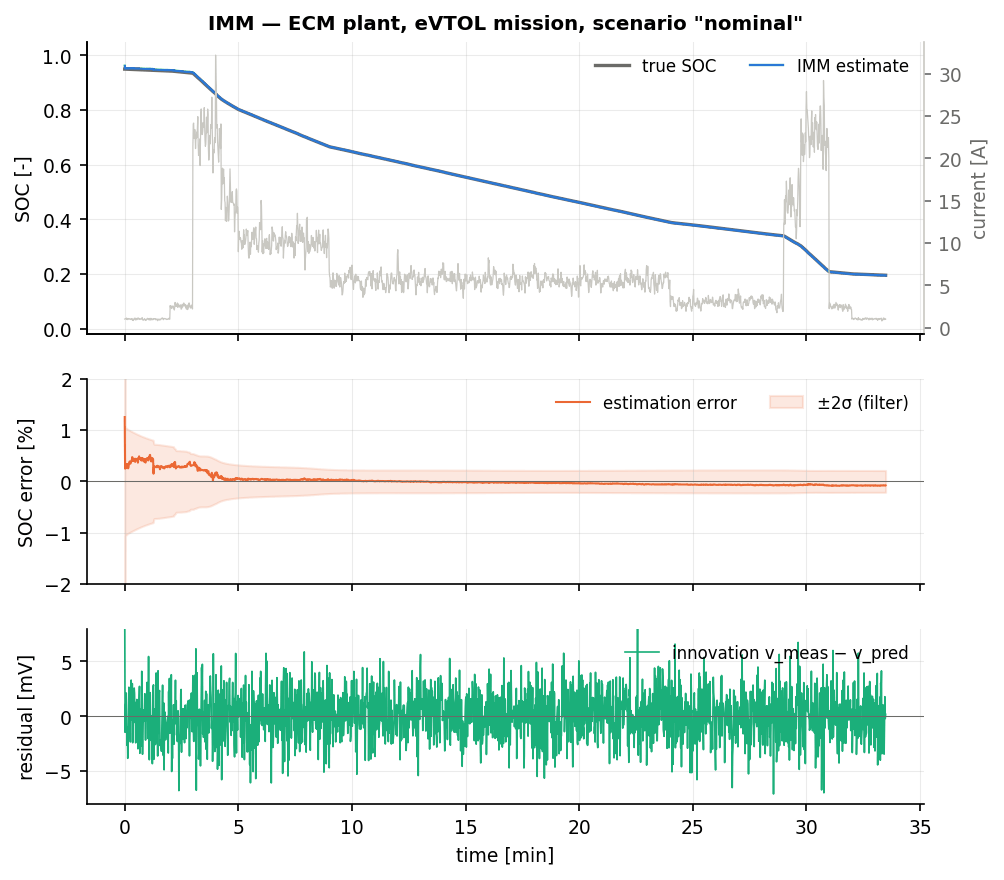
\includegraphics[width=\textwidth]{figures/cell_IMM_nominal.png}
\caption{IMM on the nominal eVTOL mission: true and estimated SOC (top), estimation error with the $\pm 2\sigma$ band when available (middle), voltage residual (bottom).}
\end{figure}
\begin{figure}[H]\centering
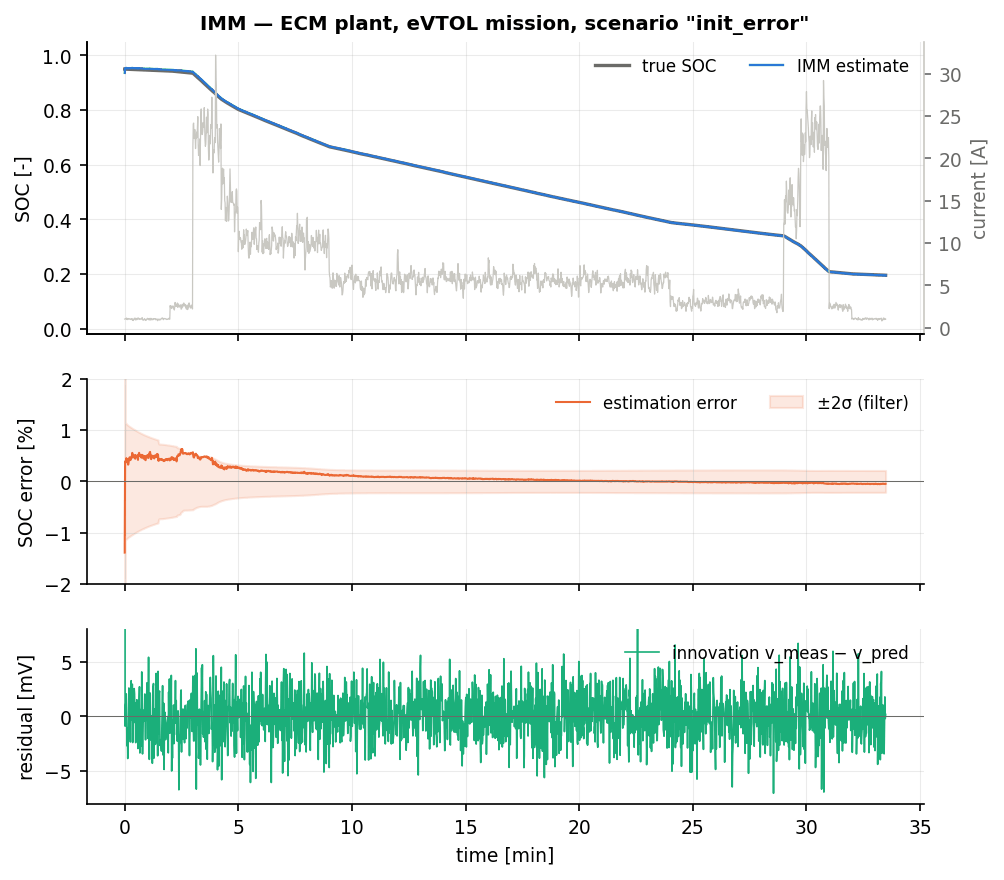
\includegraphics[width=\textwidth]{figures/cell_IMM_init_error.png}
\caption{IMM with a 35\,\% initial SOC error.}
\end{figure}
\begin{figure}[H]\centering
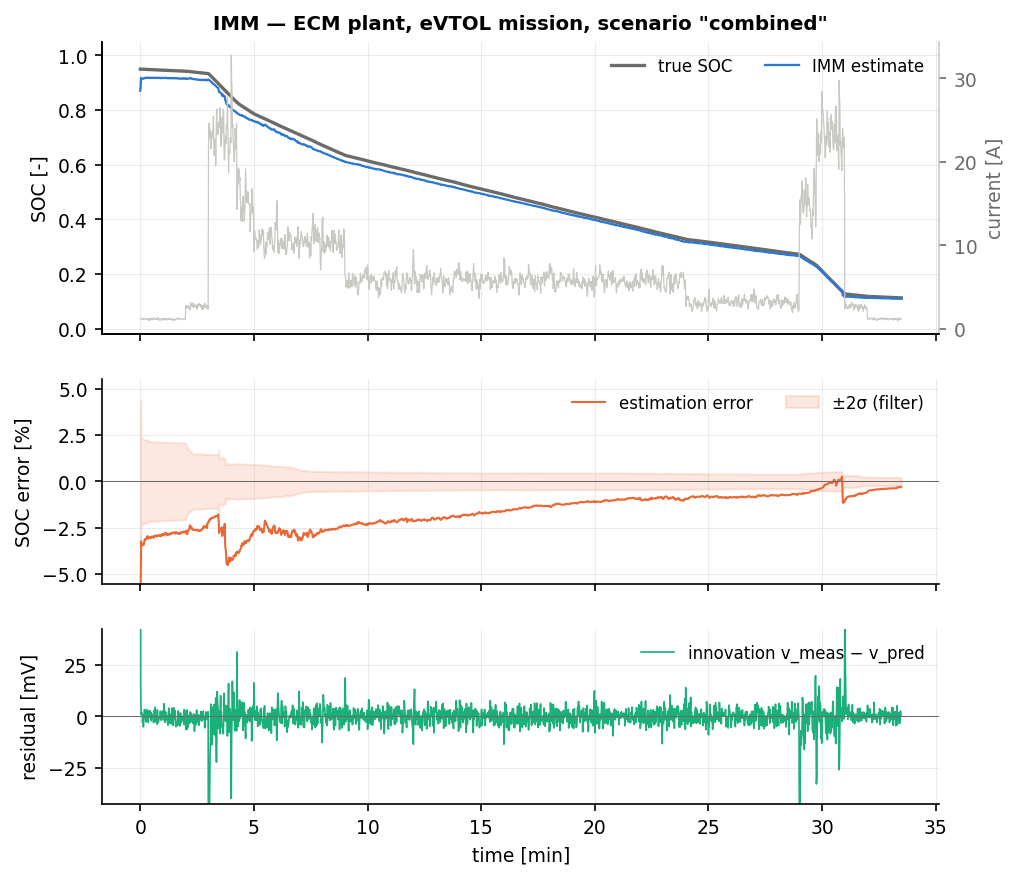
\includegraphics[width=\textwidth]{figures/cell_IMM_combined.png}
\caption{IMM on the \texttt{combined} scenario (25\,\% initial SOC error, \SI{150}{\milli\ampere} current bias, 2\,\% gain error, 10\,\% capacity loss with the associated resistance growth).}
\end{figure}
\begin{figure}[H]\centering
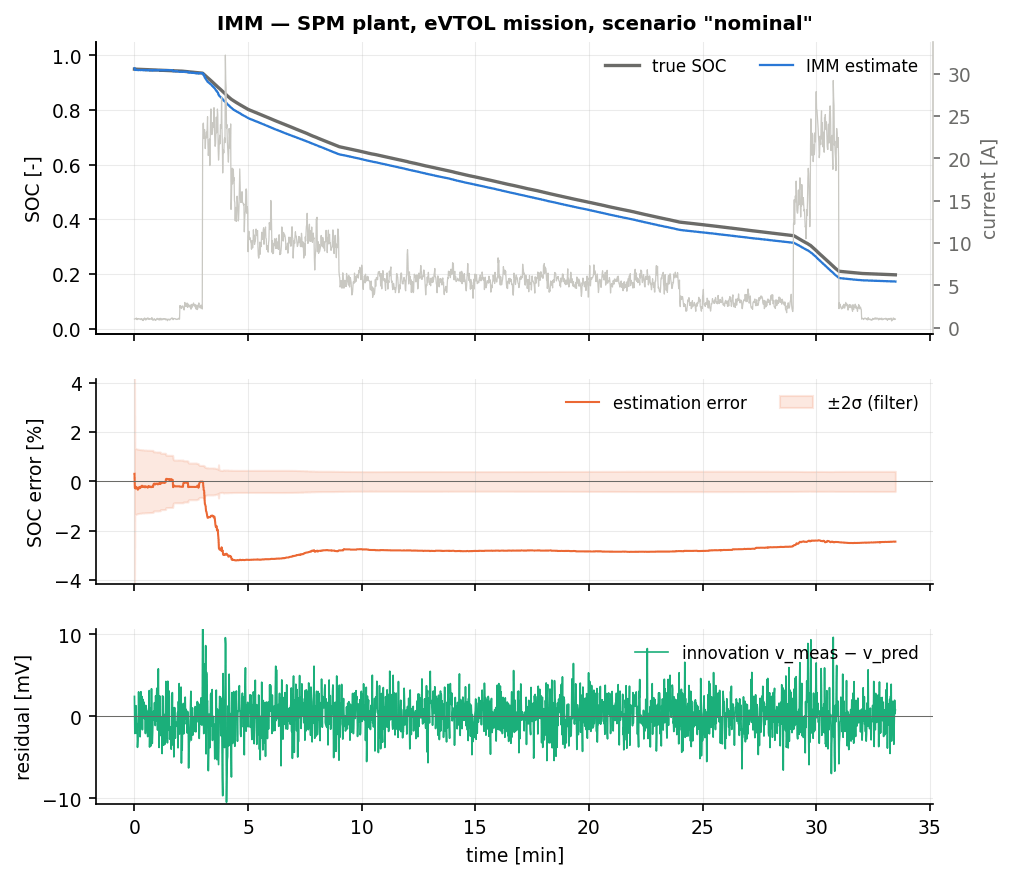
\includegraphics[width=\textwidth]{figures/cellspm_IMM_nominal.png}
\caption{IMM on the electrochemical (single-particle) plant, nominal mission: the estimator uses a 2-RC ECM fitted to that plant and therefore sees a structured \SI{4}{\milli\volt} residual instead of white noise.}
\end{figure}

All figures below are three-seed means in \% SOC, as tabulated above; the plain \texttt{EKF} run on
the same data is the reference (\texttt{EKF ref.} column).  For orientation, the EKF scores
$\mathrm{rmse}_{ss}$ = 0.05\,\% on \texttt{nominal}, 0.12\,\% on \texttt{noise\_step}, 0.21\,\% on
\texttt{outliers}, 0.46\,\% on \texttt{sensor\_dropout}, 1.36\,\% on \texttt{param\_mismatch},
1.52\,\% on \texttt{aged\_cell} and 12.44\,\% on \texttt{combined} (where it never converges), and
3.73\,\% on the nominal SPM mission.

The IMM is the most uniformly good estimator of this family: it is at least as good as the EKF on ten
of the twelve ECM scenarios and never more than $15\,\%$ worse on the other two.

\paragraph{Benign scenarios.}  \texttt{nominal}: $\mathrm{rmse}=0.18\,\%$,
$\mathrm{rmse}_{ss}=\mathbf{0.04\,\%}$ against the EKF's $0.15\,\%$ / $0.05\,\%$ --- the joint best
steady-state figure of the family.  The mode probability of the nominal hypothesis averages $0.9996$,
so the bank correctly reports that nothing is wrong.  \texttt{init\_error}: $0.16\,\%$ / $0.04\,\%$,
converging at $t=\SI{0}{\second}$ and better than the EKF on both metrics.  Both far inside the
$2\,\%$ bound.

\paragraph{Target scenario \texttt{noise\_step}.}  The IMM identifies the fault as a \emph{sensor}
problem, which is what distinguishes it from the STF.  On seed 1 the mode probability of the
degraded-voltage-channel hypothesis averages $\mu^{(2)}=1.9\times10^{-4}$ over
$t\in[100,600)\,\si{\second}$ and $\mu^{(2)}=0.989$ over $t\in[700,2010]\,\si{\second}$; the nominal
mode goes from $0.9996$ to $5.7\times10^{-4}$.  The switch is not a tuning artefact --- it is the
likelihood ratio \eqref{eq:imm:mu} doing its job --- and it is directly usable as a
"voltage-sense-channel degraded" flag.  The SOC metrics are $\mathrm{rmse}=0.18\,\%$ and
$\mathrm{rmse}_{ss}=\mathbf{0.05\,\%}$ against the EKF's $0.18\,\%$ / $0.12\,\%$, a $2.4\times$
steady-state reduction that matches the dedicated $\mR$-adaptive filters, and the voltage-prediction
error falls from \SI{2.89}{\milli\volt} to \SI{1.05}{\milli\volt}.  Contrast the STF on the same
scenario: $1.94\,\%$ / $2.34\,\%$ with $\mathrm{rmse}_v=\SI{16.04}{\milli\volt}$.  Carrying both
hypotheses is what makes the difference.

\paragraph{Target scenario \texttt{outliers}.}  $\mathrm{rmse}=0.18\,\%$,
$\mathrm{rmse}_{ss}=0.08\,\%$ against the EKF's $0.52\,\%$ / $0.21\,\%$ --- a $2.9\times$ /
$2.6\times$ improvement, with the maximum error down from $2.92\,\%$ to $1.94\,\%$ and the best
full-run RMSE of the family alongside VB-AKF ($0.12\,\%$).  The high-$\mR$ mode takes enough
probability during each burst of spikes to blunt them, even though impulsive noise is not literally
one of the three hypotheses; a mode with a heavy-tailed measurement density, or the within-sample
reweighting of \cref{ch:vbakf}, would do better still on the steady-state metric ($0.05\,\%$).

\paragraph{Target scenario \texttt{combined}.}  The EKF never reaches the $2\,\%$ band
($t_\mathrm{conv}=$ --, $\mathrm{rmse}=16.02\,\%$, $\mathrm{rmse}_{ss}=12.44\,\%$).  The IMM converges
at $t=\SI{833}{\second}$ with $\mathrm{rmse}=2.20\,\%$ and
$\mathrm{rmse}_{ss}=\mathbf{1.02\,\%}$ --- a $7.3\times$ and $\mathbf{12.2\times}$ improvement, the
best steady-state result of the whole family on this scenario (Fading-EKF $1.18\,\%$; VB-AKF
$1.87\,\%$; STF $2.71\,\%$).  What is interesting is \emph{how} it is achieved.  The mismatch mode
carries only $\mu^{(3)}\approx0.043$--$0.066$ of the probability and the nominal mode keeps
$0.91$--$0.93$, so the output is not simply "the bank switched to the right filter".  The mechanism is
the mixing step \eqref{eq:imm:P0}: because the three mode estimates disagree by a few percent of SOC,
the rank-one spread terms inflate $\mP^{0(1)}$ of the \emph{nominal} filter every single step, which
keeps its gain from collapsing.  The IMM is thus, among other things, an automatic
covariance-inflation mechanism whose inflation is driven by inter-model disagreement rather than by a
fixed factor --- a data-driven version of the fading-memory filter of \cref{ch:fadingekf}.

\paragraph{Ageing and other mismatch.}  \texttt{aged\_cell} ($15\,\%$ capacity loss, $37.5\,\%$
resistance growth): $\mathrm{rmse}$ $1.18\to\mathbf{0.66\,\%}$ and $\mathrm{rmse}_{ss}$
$1.52\to\mathbf{0.83\,\%}$, a $1.8\times$ improvement and the best of this family on that scenario ---
with $\mu^{(1)}=0.93$, $\mu^{(3)}=0.04$, again mostly through mixing.  \texttt{sensor\_dropout}:
$0.72\to0.18\,\%$, $0.46\to0.05\,\%$ ($4.0\times$ / $9.2\times$).  \texttt{param\_mismatch}:
$1.28\to0.88\,\%$, $1.36\to0.96\,\%$, with the maximum error falling from $2.87\,\%$ to the family's
lowest $1.24\,\%$.  \texttt{preisach} is a draw in steady state ($0.20\,\%$ for both, full run
$0.70\,\%$ against $0.58\,\%$) and \texttt{cold} is the one scenario where the IMM is mildly worse
($0.24\,\%$ / $0.18\,\%$ against $0.20\,\%$ / $0.16\,\%$): at $T=\SI{-10}{\celsius}$ the innovations
are strongly coloured by the slowed RC dynamics, which the likelihood reads as weak evidence for the
mismatch mode and which the mixing then converts into a little extra gain and a little extra noise.

\paragraph{Cost.}  \SI{2076}{\nano\second}/step, $4.3\times$ the EKF's \SI{478}{\nano\second} --- by
some margin the most expensive estimator of this family.  For a single cell on a modern MCU that is
irrelevant; for a 96-cell pack it is the dominant design constraint.

\paragraph{Electrochemical (SPM) plant.}  On the single-particle plant, where a 2-RC ECM leaves a
structured \SI{4}{\milli\volt} residual instead of white noise, the IMM reaches
$\mathrm{rmse}_{ss}=2.81\,\%$ on the nominal mission against the EKF's $3.73\,\%$ --- a $25\,\%$
improvement, the best of the six filters that are not purely $\mP$-inflating, but an order of
magnitude behind the Fading-EKF ($0.36\,\%$) and the STF ($0.66\,\%$).  The result is exactly what the
bank design predicts.  Two of the three hypotheses (nominal and "noisy sensor") respond to the
structured residual by keeping or lowering the gain, which hands SOC to the coulomb integrator whose
fitted capacity and efficiency are the faulty component here; only the third, which raises $q$ by a
hundred, shortens the filter's memory in the way that actually helps, and it is deliberately paired
with $\varrho_3=100$ so that half of its benefit is given back.  That pairing is the right compromise
on the ECM plant --- it is what turns \texttt{aged\_cell} from $3.71\,\%$ into $0.83\,\%$ (see
\cref{sec:imm:bank}) --- but on the SPM plant it caps the achievable gain, because under
\emph{structured} model error the correct response is unambiguously to trust the measurement more, and
the bank never commits to that hypothesis alone.  The IMM's real advantage on this plant is breadth
rather than depth: \texttt{sensor\_dropout} $5.31\to1.60\,\%$ ($3.3\times$), \texttt{current\_bias}
$5.69\to4.35\,\%$, \texttt{cold} $7.35\to2.22\,\%$ ($3.3\times$, converging in \SI{20}{\second}),
\texttt{outliers} $1.99\to2.25\,\%$ and \texttt{param\_mismatch} $3.13\to2.41\,\%$ --- it is never
badly wrong on either plant, which no single-hypothesis filter in this chapter can claim.  A bank that
included a genuine short-memory hypothesis ($q$ large, $\varrho=1$) would close most of the remaining
gap to the Fading-EKF at the cost of the ECM ageing result; that trade is the subject of
\cref{sec:imm:bank}.

\section{Summary}
The IMM is the answer to the question every other filter in this chapter begs: not "how much extra
uncertainty is there" but "\emph{what kind}".  Carrying a nominal, a noisy-sensor and a
model-mismatch hypothesis with a Markov switching prior, it matches the best dedicated
$\mR$-estimator on a tenfold voltage-noise step (and says so, with $\mu^{(2)}=0.99$), gives the
family's best steady-state result on the hardest combined-fault scenario ($12.2\times$ better than
the EKF) and on \texttt{aged\_cell} ($1.8\times$), and is the only member of this family that is
never badly wrong on either plant.  Its mode
probabilities are a health signal no single filter can produce.  Use it when several distinct
failure modes must be distinguished and $r$ filters fit the compute budget.  Do not expect it to
handle a disturbance that is not in the bank --- impulsive outliers and un-modelled hysteresis pass
straight through --- and remember that the transition matrix is a designer's assertion, not
something the data identify.
